\documentclass[conference]{IEEEtran}
\IEEEoverridecommandlockouts
% The preceding line is only needed to identify funding in the first footnote. If that is unneeded, please comment it out.
\usepackage{cite}
\usepackage{amsmath,amssymb,amsfonts}
\usepackage{algorithmic}
\usepackage{graphicx}
\usepackage{textcomp}
\usepackage{xcolor}
\usepackage{float}
\def\BibTeX{{\rm B\kern-.05em{\sc i\kern-.025em b}\kern-.08em
    T\kern-.1667em\lower.7ex\hbox{E}\kern-.125emX}}
\begin{document}

\title{Face, Gender and Age Recognition From Images Using Neural Networks\\}

\author{\IEEEauthorblockN{Ali Atahan Topal}
\IEEEauthorblockA{\textit{Isik University} \\
\textit{Computer Science}\\
Istanbul, Turkey \\
21COMP5017@isik.edu.tr}
}

\maketitle
\begin{abstract}
Face, gender and age detection are three of the big topics in the field of computer vision. In this research, the current related works and the history of face, gender and age detection will be explained and three custom models for each face, gender and age detection problems will be trained to compare with the previous researches about this topics. After the comparisons these three models will be merged to create an output that contains the detected face, gender and age.
\end{abstract}
\begin{IEEEkeywords}
Face detection, Gender classification, Age classification, SVM, ANN, CNN VGG16, MMdetection, detectron2 and SDD
\end{IEEEkeywords}

\section{Introduction}
Gender and age detection is essential for a human to interact with another human and with the help of the machine learning and deep learning methods, machines can now make these determinations that, in the past, may have only been made by humans.

\bigskip

Face detection is a hot topic in the field of computer vision, same goes for the gender and age detection from facial images. Detection of face, gender and age on images involves locating the face which is followed by estimation of the gender and age of the individual. While detecting the face the main facial features should be located, and these facial features should be used in determining the gender and the age of the person in the image.

\bigskip

All the face, gender and age detection can be used in many real life applications. Face detection is the biggest one on the three because it is a required step in the age and gender detection. Age detection could be used as a age-restricted access. It can detect the age of the user based on the image and can give the user the access based on that age. 

\bigskip

Gender detection applications can be seen in tracking and surveillance, human-computer interactions, bio-metrics, facial expression analysis. Since gender is one of the most important factors of human interaction the recognition of the gender from a machine is getting more and more important by day with the development of technology and social media.

\bigskip

In this study, deep learning based neural networks will be used to locate faces and detect the age and gender from the located face in an image.

\section{Related Works}

There are many researches about the face, age and gender detection and most of them are using deep learning techniques. Some of these deep learning techniques includes, Convolutional Neural Networks (CNN), Artificial Neural Networks (ANN) mostly and a supervised learning technique as Support Vector Machines (SVM). 
\bigskip

SVM is a supervised learning method commonly used for both classification and regression. It can plot every item as a point and each features value will be the coordinate in the n-dimensional space.

\bigskip
ANNs are biologically inspired simulations on tasks like clustering, classifications, pattern recognition that computers perform to solve complex problems. Like other machine learning algorithms, the problems that have been solved using ANNs are varies from subject to subject. 

\bigskip

CNNs are a class of artificial neural networks that is mostly used in complex problems like image processing, image analysing, image and video recognition, image classification, image segmentation. It can be used in Natural Language Processing (NLP) as well. Overall CNN is a strong tool for visual imagery.

\bigskip

In one of the research the face detection rate using single network with no heuristics and 2 copies of hidden units, 2905 connections was the highest with 99.6\% detection rate. Single network with heuristics that has a threshold(2,1) and overlap elimination was the highest among the models with heuristics has 99.5\% detection rate. The highest detection rate was achieved while arbitration among two networks with 99.7\% detection rate. To train this model they selected and used nearly 1050 face examples from the CMU and Harvard databases. These face images contained various sizes, orientations, positions and intensities. \cite{b1}

\bigskip

Another research that used CNNs achieved a good face, age and gender detection from images but there were no detection rates only images of the face detection and some predictions. The dataset used in this research was found in Kaggle and consists of 26580 photos of 2284 individuals. \cite{b5}

\bigskip

Only for gender detection from images CNNs and The local Recetive Field-Extreme Learning Machine was used and the accuracy of gender classification is 87.13\% and 80\% respectively. In this research a dataset that was made in 2014 via smartphones used. This dataset contained approximately 2000 individual's faces and the total image count was around 26000. They split this dataset to two groups which is faces and straight faces. The straight faces group was selected to be used. There are 13239 images but the gender and age of babies and children are hard to predict these kind of images were not involved in the research.\cite{b2}

\bigskip

Only for age detection a work scheme of image - preprocessing - feature extraction - SVM was used. The database used for this research was the fusion of the FG-NET Aging database and Adience benchmark of unfiltered faces for gender and age classification which formed 26580 photos from 2284 subject. After the experimentation results of testing older than 20 years old was the highest with 71.102\% and the older than 32 years old was following with 61.066\%. \cite{b3}

\bigskip

All of the related works using similar data and similar image counts around 26000 images from 2000 individuals but the methods they use are not the same. The results of these researches are close but again not same.

\section{Approach}

Face detection is a big topic in computer science. The reason being the usage of face detection in real world scenarios. In this research we will detect face, age and gender but for age and gender we need a deep learning model that detects faces accurately. For object detection there are many pre-trained models such as MMdetection, detectron2, SDD(Single Shot Detector), R-CNN's etc.

\bigskip

We used the LFW (The Labeled Faces in the Wild) dataset in our experiments.  From LFW random 95 images were selected and 5 more images added as a non face class. For total 100 images were selected. To train a model to detect object the model needs a annotation for where the object is to annotate the selected 100 images a library called labelme was used. After annotation the 100 images were randomly selected and splited to train, test and validation sets with their annotations for 70\%, 15\% and 15\% respectively. Since 100 images are not enough to train a deep learning model, the selected images were augmented with random crops, random brigtness, random gamma, horizontal and vertical flips, random RGB shifts to create 60 times more images with a library called albumentations which does the annotations of the augmented images for us automatically.

\bigskip

After the augmentations of the images now the total image count is 6000 which is enough to train a deep learning model. The train set has 4080, test and validation set has 900 images respectively. To create the train, test and validation sets which will be used as the inputs for the deep learning model the images and labels were read and combined as a TensorFlow dataset.

\bigskip

In this research the model that is used as a baseline is VGG16 model which is used in SDD model as well. 

\begin{figure}[htbp]
\centering
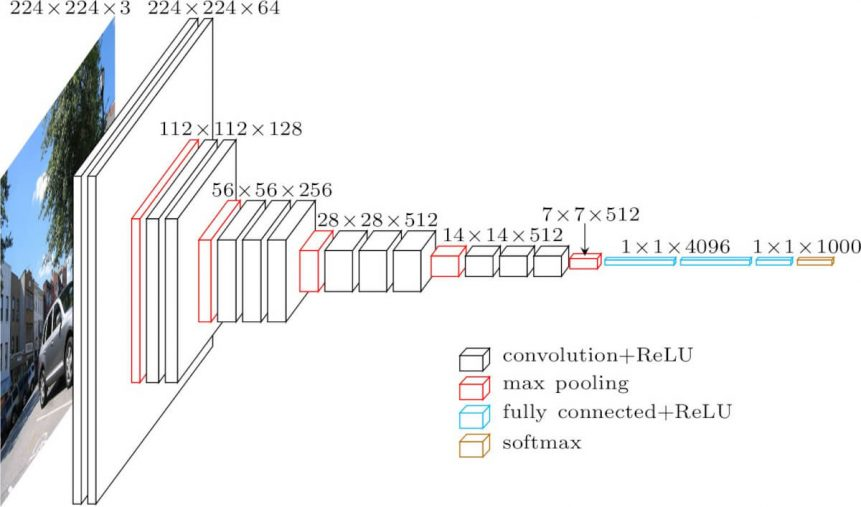
\includegraphics[scale=0.39]{VGG16-model.jpg}
\caption{VGG16 Model}
\label{fig:VGG16}
\end{figure}

\bigskip

VGG16 model is a combination of 16 layers that have weights. The 16 comes from the layer count. It contains 13 Convolutional layers, 5 Max Pooling layers and 3 Dense layers which makes it have 21 layers in total. Face detection has two problems one is whether the image has a face which is a classification problem and if the image has a face where is the face's coordinates, and this is a regression problem. 

\bigskip

To solve the classification and regression problems VGG16's top 3 dense layers were not used and instead of them 1 GlobalMaxPooling2D layer connected to 2 Dense layers for classification output and same for regression output were used. 

\begin{figure}[htbp]
\centering
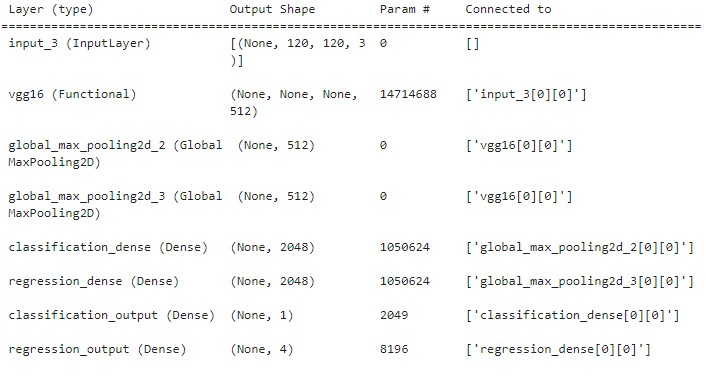
\includegraphics[scale=0.50]{Model_summary.jpg}
\caption{Used Model Summary}
\label{fig:ModelSummary}
\end{figure}

\bigskip

Adam optimizer was used with a learning rate of 0.0001. Since there is two problem and 2 output of the model there is a need of two loss functions. For the classification loss Binary Crossentropy was used but for the regression loss a new loss function was written for measuring the Localization Loss.[Fig. \ref{fig:LocalizationLoss}]

\begin{figure}[htbp]
\centering
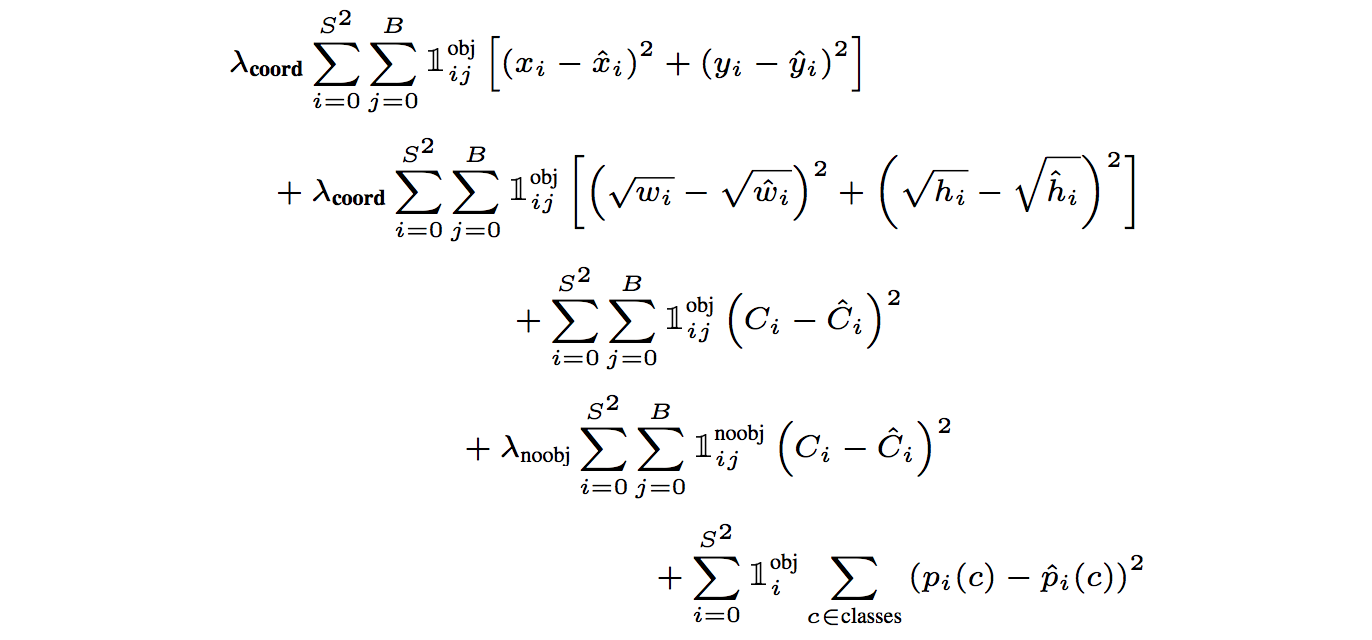
\includegraphics[scale=0.20]{Localization Loss.png}
\caption{Localization Loss}
\label{fig:LocalizationLoss}
\end{figure}

\bigskip

And the model trained for 15 epochs and 510 batches for epoch. With a RTX 3060 GPU and took around 5-8 minutes to train.

\bigskip

After the face detection we need two more models to classify wheter the detected image is a Female or Male and after that comes the age classification. For both gender and age classifications a dataset callds UTKFace was used. It consists over 20000 images that have only one cropped face per image and the images are labelled in by their name in [age]\_[gender]\_[ethnicity]\_[datetime].jpg format. 
This images were read and created a dataframe with columns of Image, Gender and Age.
After the creation of this a brief analysis of the dataset was performed. As a result of this analysis the number of images that are between 0-4 age was so high. So the \%30 percentage of 0-4 age were removed from the dataset to ensure the model's training is not overfitting. 

\bigskip

After a CNN with 1 input layer, 4 Convolutional2D layers and 4 MaxPooling2D layers in between Convolutional2D layers followed by a flatten layer then a dense dropout layer and finally an output layer was created and trained for 9 epochs with 64 batch size.[Fig. \ref{fig:Gendermodelsummary}]

\begin{figure}[htbp]
\centering
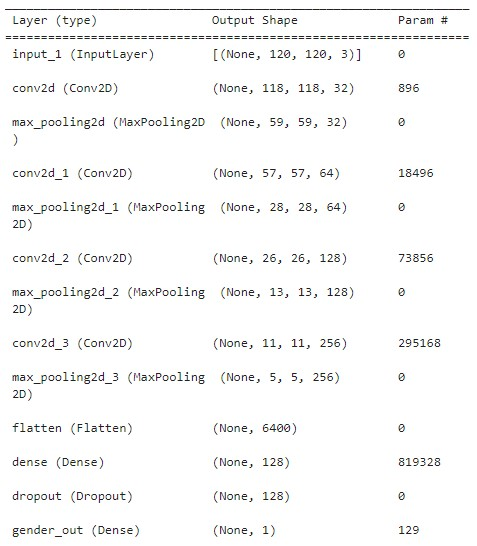
\includegraphics[scale=0.60]{gendermodelsummary.jpg}
\caption{Gender Model Summary}
\label{fig:Gendermodelsummary}
\end{figure}

\bigskip

For the age classification the dataset was splited to 6 classes that are 
(0-14), (15-25), (26-40), (41-65), (66-100), (101+). And a CNN model with convolutional2D, MaxPooling2D, Dropout, Dense and Flatten layers and trained for 25 epochs with 64 batch size.[Fig. \ref{fig:Agemodelsummary}]

\begin{figure}[htbp]
\centering
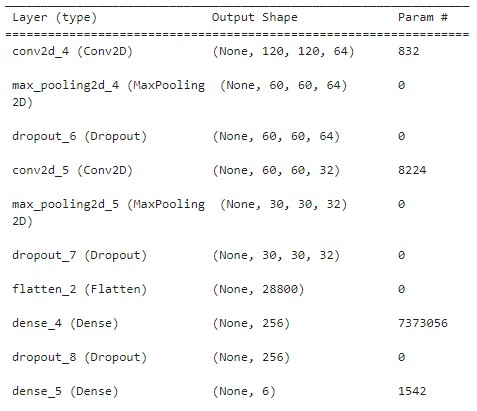
\includegraphics[scale=0.65]{agemodelsummary.jpg}
\caption{Age Model Summary}
\label{fig:Agemodelsummary}
\end{figure}


\section{Results}

While training the face detection model we had total loss, classification loss, regression loss and most of the time they were decreasing for each epoch which is a good sign that shows the model is actually learning. When we plot the losses;

\begin{figure}[htbp]
\centering
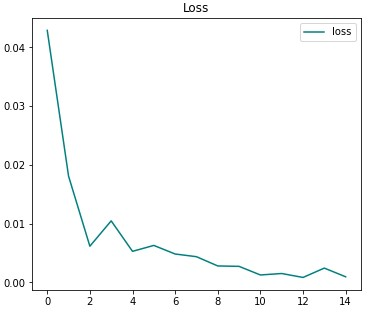
\includegraphics[scale=0.75]{total_loss.jpg}
\caption{Total Loss}
\label{fig:TotalLoss}
\end{figure}

\begin{figure}[htbp]
\centering
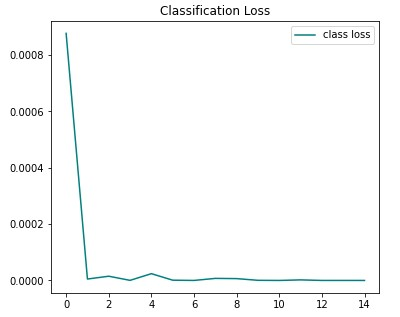
\includegraphics[scale=0.75]{classification_loss.jpg}
\caption{Classification Loss}
\label{fig:ClassificationLoss}
\end{figure}

\begin{figure}[htbp]
\centering
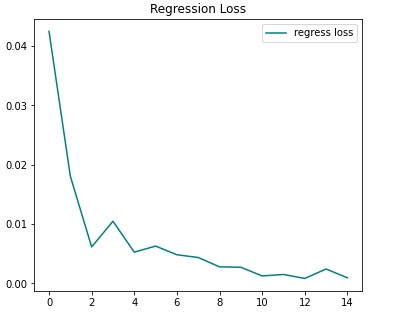
\includegraphics[scale=0.75]{regression_loss.jpg}
\caption{Regression Loss}
\label{fig:RegressionLoss}
\end{figure}

We can see that the total loss, classification loss and regression loss were constantly dropping. There are some little bumps here and there but generally model seems to learn just fine. 

\begin{figure}[htbp]
\centering
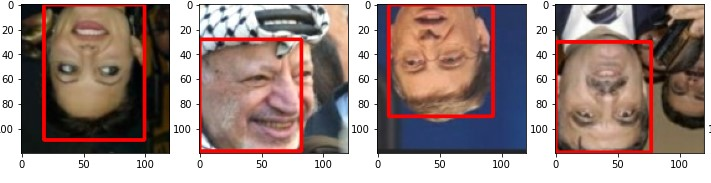
\includegraphics[scale=0.45]{pred1.jpg}
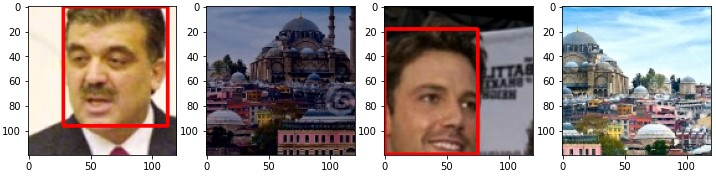
\includegraphics[scale=0.45]{pred2.jpg}
\caption{Test data predictions}
\label{fig:Predictions}
\end{figure}

\bigskip

As for the predictions the model seems to detect faces nicely and in the images where there is no face the model detects that it is not a face class so there is no bounding boxes for the faces. 

\bigskip

For calculating the face detection accuracy we need two values. One for the classification and one for the regression. For classification the model recognizes that there is a face in the image with \%99.5 accuracy in total 900 images. As for the regression part we used intersection over union and took the average of the detected faces for the mean average precision. Intersection over union is a metric that has been used for calculating the accuracy of the object detection models. 

\begin{figure}[htbp]
\centering
\includegraphics[scale=0.50]{Iou.jpg}
\caption{Intersection Over Union}
\label{fig:IoU}
\end{figure}

After the calculation the mean average precision of the face detection model came out to be \%73.17.

\begin{figure}[htbp]
\centering
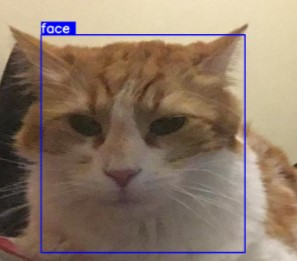
\includegraphics[scale=0.75]{cat.jpg}
\caption{Cat}
\label{fig:Cat}
\end{figure}

\bigskip

The model seems to work on cats as well.

\bigskip

As for the gender classification model, we had binary cross-entropy as a loss function since gender is a binary variable. When we plot the losses and the accuracy for the gender classification model we can see that the model learning the features of the images, the loss and the accuracy is getting effected positively.

\begin{figure}[htbp]
\centering
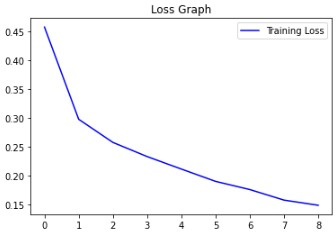
\includegraphics[scale=0.75]{gender_loss.jpg}
\caption{Gender Classification Model Loss}
\label{fig:genderloss}
\end{figure}

\begin{figure}[htbp]
\centering
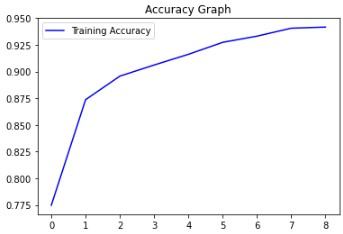
\includegraphics[scale=0.75]{gender_accuracy.jpg}
\caption{Gender Classification Model Accuracy}
\label{fig:genderaccuracy}
\end{figure}

\bigskip
In the testing phase of this model the test part of the UTKFace model was used and in gender classification the model reached \%93.8 accuracy classifying the gender of the person in the image.

The age classification the model wasn't as accurate as the gender model but it was enough since the age classification is the hardest problem out of the face detection, gender classification and age classification. 

We can see from the loss and accuracy graph the age model started to learn the features of the dataset but the learning accuracy was reaching a stalemate around \%75. With using the test part of the UTKFace, the age classification model reached \%73.86 accuracy on predicting the age group of the person.

\begin{figure}
\centering
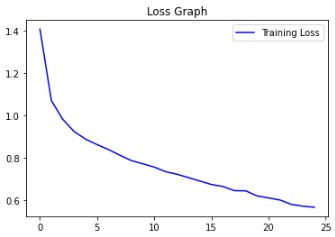
\includegraphics[scale=0.75]{age_loss.jpg}
\caption{Age Classification Model Loss}
\label{fig:ageloss}
\end{figure}

\begin{figure}
\centering
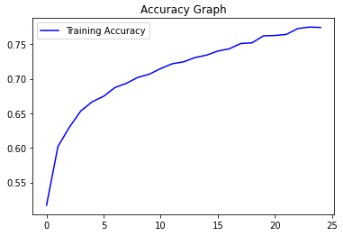
\includegraphics[scale=0.75]{age_accuracy.jpg}
\caption{Age Classification Model Accuracy}
\label{fig:ageaccuracy}
\end{figure}

Here are some predictions of the gender and age classification models. 


\begin{figure}[H]
\centering
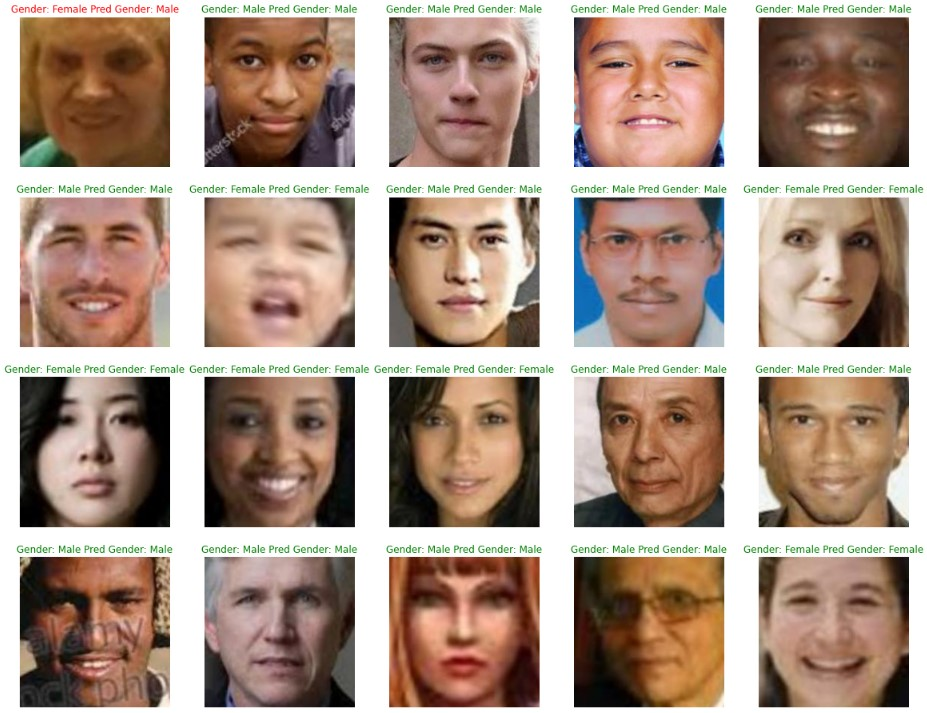
\includegraphics[scale=0.33]{gender_pred.jpg}
--------------------------------------------------------------------
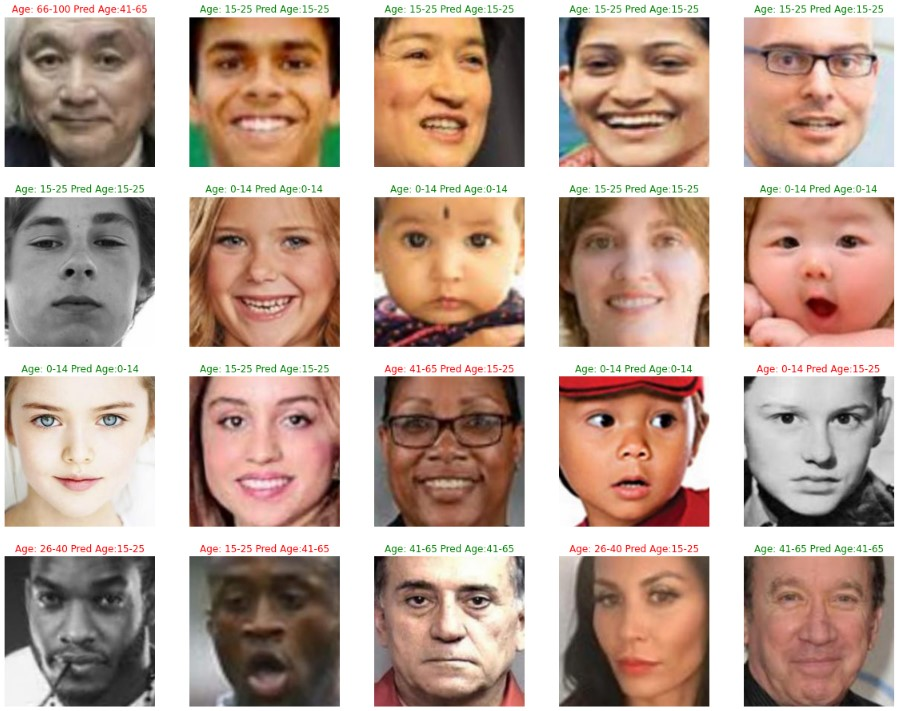
\includegraphics[scale=0.33]{age_pred.jpg}
\caption{Gender and Age Classification Model Predictions}
\label{fig:genderpred}
\end{figure}

After the tests of all the three models we got the final model as a service with the combination of these three. The final model detects the face in the given image after that it crops the given image from the coordinates, then the gender and age classification models use the cropped image to predict the value for the cropped image.
    
\bigskip

\section{Conclusion}

With the usage of Deep Learning the trained models were able to detect that there is a face in the image with \%99.5 accuracy. As for the gender classification the trained model reached \%93.8 accuracy which is good still. The hardest problem out of the face detection, gender detection and age detection is the age detection for this problem we used age intervals as classes and trained the model with those intervals as the output. The trained model was able to reach \%73.86 accuracy.

\bigskip
Some predictions from the final model.

\begin{figure}[htbp]
\centering
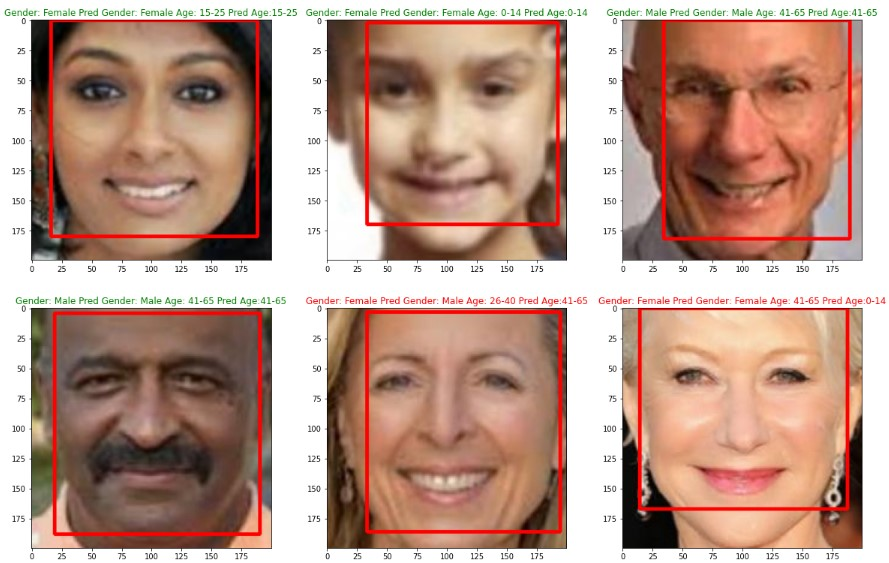
\includegraphics[scale=0.33]{finalmodel.jpg}
\caption{Final Model Predictions}
\label{fig:finalmodel}
\end{figure}


\bigskip

\begin{thebibliography}{00}
\bibitem{b1} H. A. Rowley, S. Baluja and T. Kanade, "Neural network-based face detection," in IEEE Transactions on Pattern Analysis and Machine Intelligence, vol. 20, no. 1, pp. 23-38, Jan. 1998, doi: 10.1109/34.655647.
\bibitem{b2} Y. Akbulut, A. Şengür and S. Ekici, "Gender recognition from face images with deep learning," 2017 International Artificial Intelligence and Data Processing Symposium (IDAP), 2017, pp. 1-4, doi: 10.1109/IDAP.2017.8090181.
\bibitem{b3} V. Almeida, M. K. Dutta, C. M. Travieso, A. Singh and J. B. Alonso, "Automatic age detection based on facial images," 2016 2nd International Conference on Communication Control and Intelligent Systems (CCIS), 2016, pp. 110-114, doi: 10.1109/CCIntelS.2016.7878211.
\bibitem{b4} A. S. Al-Shannaq and L. A. Elrefaei, "Comprehensive Analysis of the Literature for Age Estimation From Facial Images," in IEEE Access, vol. 7, pp. 93229-93249, 2019, doi: 10.1109/ACCESS.2019.2927825.
\bibitem{b5} A. Saxena, P. Singh and S. Narayan Singh, "Gender and Age detection using Deep Learning," 2021 11th International Conference on Cloud Computing, Data Science \& Engineering (Confluence), 2021, pp. 719-724, doi: 10.1109/Confluence51648.2021.9377041.
\end{thebibliography}

\end{document}
